\chapter{Оптимизация параметров}\label{optimization}
Код FAINA позволяет не только расчитывать излучение заданных источников, но и фитировать наблюдательные данные модельными, подбирая необходимые параметры. Реализованы методы оптимизации, пригодные для произвольного числа параметров и широкого класса моделей источников. В качестве целевой функции используется взвешенная сумма квадратов отклонений по всем наблюдательным точкам $f = \sum \frac{(F_i - F_{obs,i})^2}{\sigma_i^2}$, где $F_i$ - расчетная спектральная плотность потока излучения, $F_{obs,i}$ - наблюдаемая спектральная плотность потока излучения, $\sigma_i$ - её погрешность. 

Реализованные методы оптимизации делятся на два типа - те, которые рассматривают излучение в один момент времени, либо постоянные во времени, и те, которые учитывают эволюцию источников и используют наблюдения в разные моменты времени. В последнем случае пользователю необходимо самостоятельно указывать, как меняются параметры источника со временем, см. \ref{timeDependentSource}.

\section{Фитирование источников, не зависящих от времени}
Для фитирования постоянных во времени кривых блеска предназначен абстрактный класс RadiationOptimizer. В нем определена виртуальныя функция optimize(double* vector, bool* optPar, double* nu, double* observedInu, double* observedError, int Nnu, RadiationSource* source), которая и производит процесс оптимизации. Входными параметрами являются: vector - массив подбираемых параметров, в который будет записан результат работы программы, optPar - массив булевских переменных, определяющих оптимизировать соответствующий параметр, или ситать его фиксированным, nu - массив энергий, на которых производились наблюдения, observedInu - соответствующие наблюдаемые потоки в единицах $\text{см}^{-2}\text{с}^{-1}$, Nnu - количество наблюдательных точек, source - источник излучения. Функция изменения параметров источника source->resetParameters, описанная в разделе \ref{sourcesSection}, должна быть согласована с массивом оптимизируемых параметров vector, так как в процессе оптимизации он будет передаваться в нее в качестве входного параметра.

В коде реализованы два наследника класса RadiationOptimazer: GridEnumRadiationOptimizer - производящий поиск минимума простым перебором по сетке параметров, и GradientDescentRadiationOptimizer - в котором минимум достигается градиентным спуском. Эти два класса полезно использовать совместно, используя результат работы первого как начальную точку для второго. Схема насследования классов оптимизаторов показана на рисунке \ref{radiationOptimizer}, а список их публичных методов приведен в Таблице \ref{RadiationOptimizerMethods}.
\begin{figure}
	\centering
	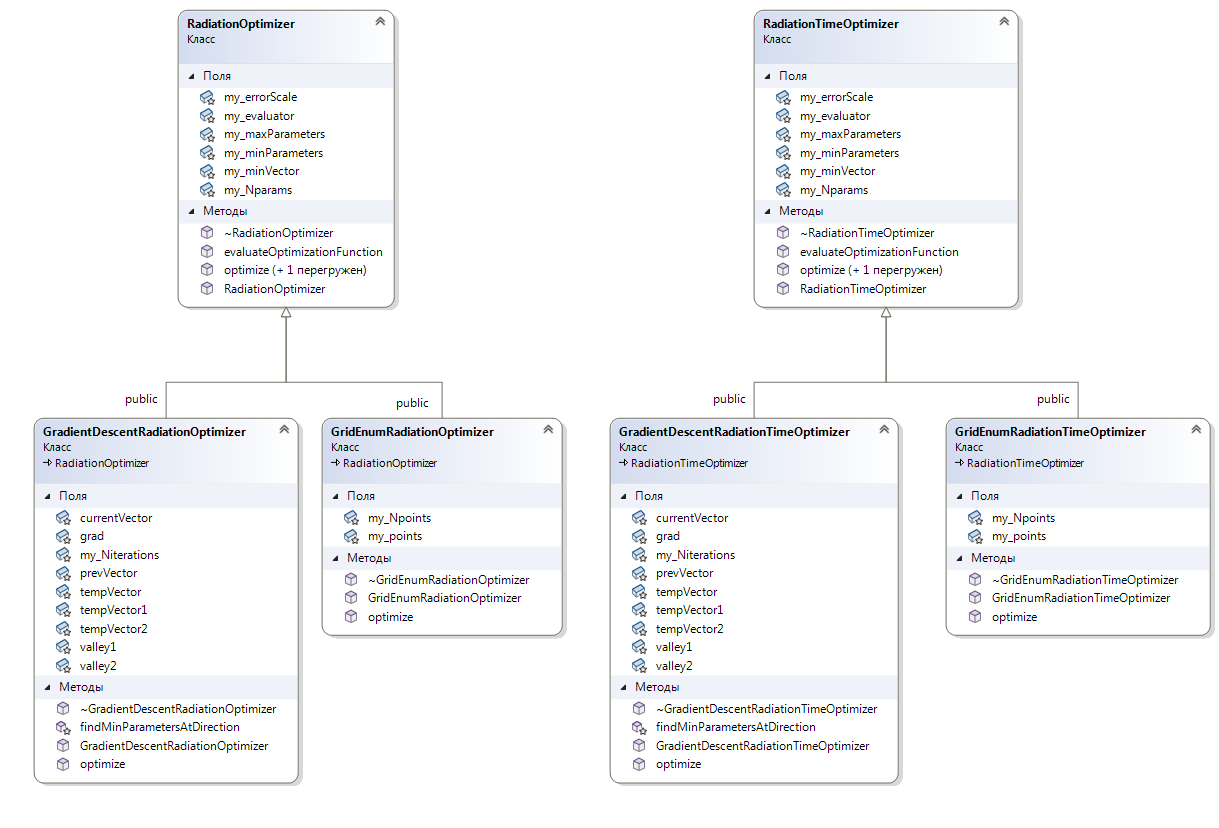
\includegraphics[width=10.5 cm]{./fig/radiationOptimizer.png} 
	\caption{Схема наследования классов оптимизаторов}
	\label{radiationOptimizer}
\end{figure}

\begin{small}
	\topcaption{Публичные методы классов оптимизаторов параметров источников }
	\label{RadiationOptimizerMethods}
	\begin{xtabular}{|p{0.5\textwidth}|p{0.5\textwidth}|}
		\hline
		\textbf{RadiationOptimizer} & абстрактный класс для оптимизации параметров источника \\
		\hline
		evaluateOptimizationFunction( const double* vector, double* nu, double* observedInu, double* observedError, int Nnu, RadiationSource* source) & \\
		\hline
		optimize( double* vector, bool* optPar, double* nu, double* observedInu, double* observedError, int Nnu, RadiationSource* source) & \\
		\hline
		optimize( double* vector, bool* optPar, double* nu, double* observedInu, int Nnu, RadiationSource* source) & \\
		\hline
		\textbf{GridEnumRadiationOptimizer} & \\
		\hline
		GridEnumRadiationOptimizer( RadiationEvaluator* evaluator, const double* minParameters, const double* maxParameters, int Nparams, const int* Npoints) & \\
		\hline
		\textbf{GradientDescentRadiationOptimizer} & \\
		\hline
		GradientDescentRadiationOptimizer( RadiationEvaluator* evaluator, const double* minParameters, const double* maxParameters, int Nparams, int Niterations) & \\
		\hline		
	\end{xtabular}
\end{small}

\section{Фитирование источников, зависящих от времени}
\begin{figure}
	\centering
	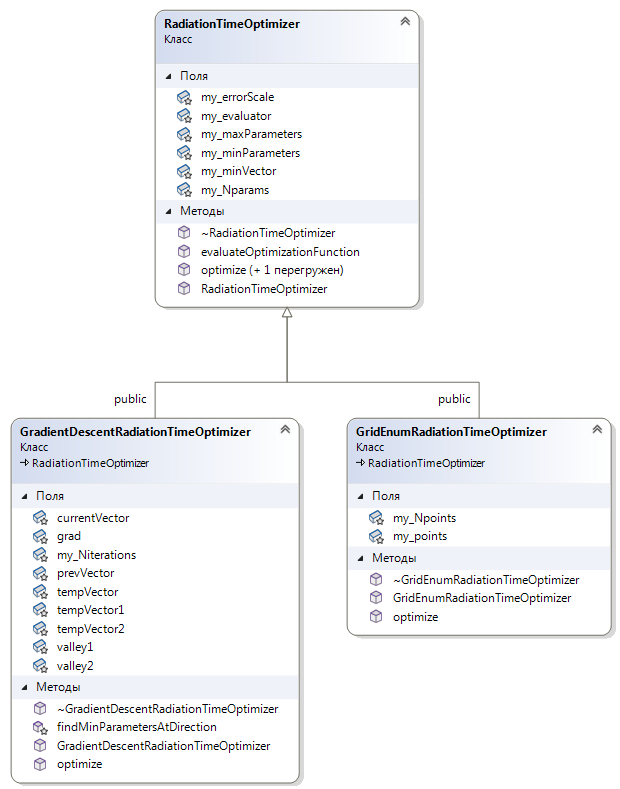
\includegraphics[width=10.5 cm]{./fig/radiationOptimizerTime.png} 
	\caption{Схема наследования классов оптимизаторов, зависящих от времени}
	\label{radiationOptimizerTime}
\end{figure}
